% Figure 1 of "Galashin's Conjecture 4.3 via a convex gradient": the proof architecture.
% Source of the figure, typeset in the paper's own fonts (T1, Latin Modern, 11pt) at the paper's text
% width (6.5in), so \includegraphics does not rescale it. Illustrates CLH-1 to CLH-5; it adds no assertion.
% Build: pdflatex <this file> && pdftocairo -svg <this file>.pdf <this file>.svg
\documentclass[11pt]{standalone}
\usepackage[T1]{fontenc}
\usepackage{lmodern}
\usepackage{amsmath,amssymb}
\usepackage{tikz}
\usetikzlibrary{arrows.meta,positioning,calc}

% the palette of the paper's other figures: blue solid for the first strand or arc, ochre dashed for the second
\definecolor{ink}{HTML}{233740}
\definecolor{muted}{HTML}{65757D}
\definecolor{pblue}{HTML}{0072B2}
\definecolor{qochre}{HTML}{B87827}

\tikzset{
  base/.style={draw=muted, line width=0.5pt},
  exit/.style={circle, draw=ink, fill=white, line width=0.6pt, inner sep=0pt, minimum size=4.6pt},
  entry/.style={circle, draw=ink, fill=ink, line width=0.6pt, inner sep=0pt, minimum size=4.6pt},
  exitP/.style={exit, draw=pblue}, entryP/.style={entry, draw=pblue, fill=pblue},
  exitQ/.style={exit, draw=qochre}, entryQ/.style={entry, draw=qochre, fill=qochre},
  strandP/.style={pblue, line width=1.1pt, -{Stealth[length=5pt,width=4.2pt]}, shorten >=2.4pt},
  strandQ/.style={qochre, line width=1.1pt, dash pattern=on 4pt off 1.6pt, -{Stealth[length=5pt,width=4.2pt]}, shorten >=2.4pt},
  lab/.style={font=\footnotesize, inner sep=1.2pt, text=ink},
  labm/.style={font=\small, inner sep=1.2pt, text=ink},
  labP/.style={font=\small, inner sep=1.2pt, text=pblue},
  labQ/.style={font=\small, inner sep=1.2pt, text=qochre},
  muted text/.style={text=muted},
  ttl/.style={font=\small, text=ink, inner sep=0pt},
  negE/.style={font=\small, text=pblue, inner sep=0pt},
  posE/.style={font=\small, text=qochre, inner sep=0pt},
  zeroE/.style={font=\small, text=ink, inner sep=0pt},
  idx/.style={font=\footnotesize, text=muted, inner sep=0pt},
}
\tikzset{
  fwd/.style={pblue, line width=1.1pt, -{Stealth[length=5.5pt,width=4.5pt]}},
  inv/.style={qochre, line width=1.1pt, -{Stealth[length=5.5pt,width=4.5pt]}},
  aux/.style={muted, line width=0.8pt, -{Stealth[length=5pt,width=4pt]}},
  obj/.style={font=\large, text=ink, inner sep=1pt},
  note/.style={font=\footnotesize, text=muted, inner sep=1pt, align=center},
  mapl/.style={font=\small, inner sep=2pt},
  stepn/.style={font=\small, text=ink, inner sep=1.5pt},
  steps/.style={font=\footnotesize, text=muted, inner sep=1pt},
}

\begin{document}
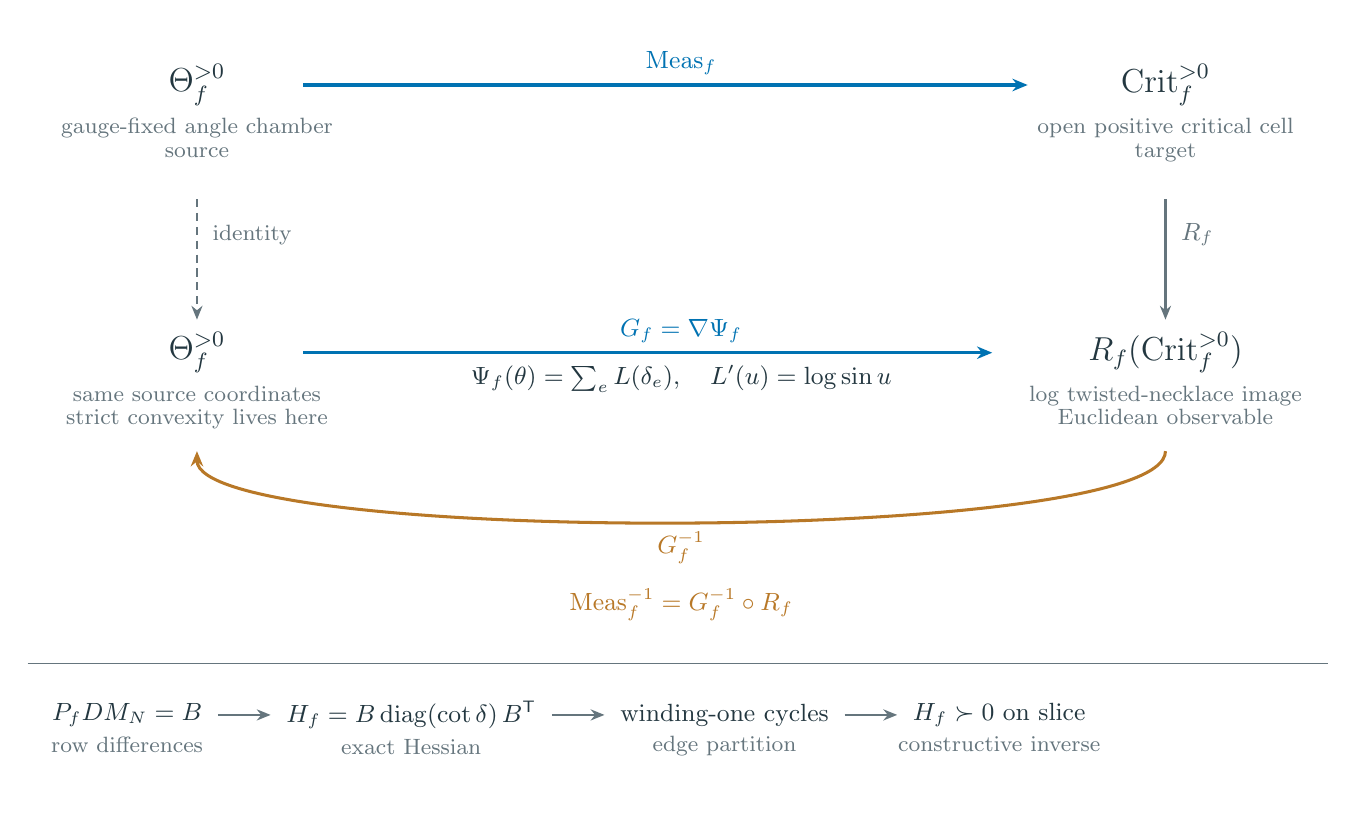
\begin{tikzpicture}[x=1cm,y=1cm]
\useasboundingbox (-0.25000,-0.62800) rectangle (16.26000,9.27800);
\node[obj] (o1) at (1.900,8.550) {$\Theta_f^{>0}$}; %t o1
\node[note, anchor=north] (o1n) at (1.900,8.170) {gauge-fixed angle chamber\\[-1pt]source}; %t o1-note
\node[obj] (o2) at (14.200,8.550) {$\mathrm{Crit}_f^{>0}$}; %t o2
\node[note, anchor=north] (o2n) at (14.200,8.170) {open positive critical cell\\[-1pt]target}; %t o2-note
\node[obj] (o3) at (1.900,5.150) {$\Theta_f^{>0}$}; %t o3
\node[note, anchor=north] (o3n) at (1.900,4.770) {same source coordinates\\[-1pt]strict convexity lives here}; %t o3-note
\node[obj] (o4) at (14.200,5.150) {$R_f(\mathrm{Crit}_f^{>0})$}; %t o4
\node[note, anchor=north] (o4n) at (14.200,4.770) {log twisted-necklace image\\[-1pt]Euclidean observable}; %t o4-note
\draw[fwd] (3.250,8.550) -- (12.450,8.550); %a Meas
\node[mapl, text=pblue, anchor=south] at (8.050,8.600) {$\mathrm{Meas}_f$}; %t meas
\draw[fwd] (3.250,5.150) -- (12.000,5.150); %a G
\node[mapl, text=pblue, anchor=south] at (8.050,5.200) {$G_f=\nabla\Psi_f$}; %t g
\node[mapl, text=ink, anchor=north] at (8.050,5.070) {$\Psi_f(\theta)=\sum_e L(\delta_e),\quad L'(u)=\log\sin u$}; %t psi
\draw[aux, dash pattern=on 3pt off 2pt] (1.900,7.100) -- (1.900,5.570); %a identity
\node[mapl, text=muted, anchor=west] at (2.020,6.650) {\footnotesize identity}; %t identity
\draw[aux] (14.200,7.100) -- (14.200,5.570); %a R
\node[mapl, text=muted, anchor=west] at (14.320,6.650) {$R_f$}; %t R
\draw[inv] (14.200,3.900) to[out=-90,in=-90,looseness=0.25] node[mapl, text=qochre, below=1pt, pos=0.5] {$G_f^{-1}$} (1.900,3.900); %a Ginv
\node[font=\small, text=qochre, inner sep=1pt] at (8.050,1.950) {$\mathrm{Meas}_f^{-1}=G_f^{-1}\circ R_f$}; %t measinv
\draw[muted, line width=0.4pt] (-0.250,1.200) -- (16.260,1.200);
\node[stepn, anchor=west] (s1) at (0.0,0.550) {$P_fDM_N=B$}; %t s1
\node[steps, below=0.03cm of s1] {row differences}; %t s1-note
\node[stepn, right=0.95cm of s1] (s2) {$H_f=B\operatorname{diag}(\cot\delta)\,B^{\mathsf T}$}; %t s2
\node[steps, below=0.03cm of s2] {exact Hessian}; %t s2-note
\draw[aux, shorten <=4pt, shorten >=4pt] (s1.east) -- (s2.west); %a s1-s2
\node[stepn, right=0.95cm of s2] (s3) {winding-one cycles}; %t s3
\node[steps, below=0.03cm of s3] {edge partition}; %t s3-note
\draw[aux, shorten <=4pt, shorten >=4pt] (s2.east) -- (s3.west); %a s2-s3
\node[stepn, right=0.95cm of s3] (s4) {$H_f\succ0$ on slice}; %t s4
\node[steps, below=0.03cm of s4] {constructive inverse}; %t s4-note
\draw[aux, shorten <=4pt, shorten >=4pt] (s3.east) -- (s4.west); %a s3-s4
\end{tikzpicture}
\end{document}
